\documentclass[a4paper,12pt]{report}
\addtolength{\oddsidemargin}{-1.cm}
\addtolength{\textwidth}{2cm}
\addtolength{\topmargin}{-2cm}
\addtolength{\textheight}{3.5cm}
\newcommand{\HRule}{\rule{\linewidth}{0.5mm}}
\setcounter{secnumdepth}{5}
\setcounter{tocdepth}{3}
\makeindex

\usepackage{longtable}
\usepackage{graphicx}
\usepackage{makeidx}
\usepackage{hyperref}
\usepackage{verbatim}
\usepackage{placeins}

\hypersetup{
    colorlinks=true,
    linkcolor=blue,
    filecolor=magenta,      
    urlcolor=cyan,
}


% define the title
\author{Ambitious Design}
\title{ Software Requirements Specifications and Technology Neutral Process Design}
\begin{document}
\setlength{\parskip}{6pt}

% generates the title
\begin{titlepage}

\begin{center}
% Upper part of the page           
\textsc{\LARGE Willburg Outdoor PTY(ltd.)}\\[1.5cm]
\textsc{\Large Smart Image Identifier }\\[1.0cm]
\textsc{\Large Version 1.0 }\\[0.5cm]
% Title
\HRule \\[0.4cm]
{ \huge \bfseries  Application Requirements Specifications and Design}\\[0.4cm]
\HRule \\[0.4cm]
% Author and supervisor
\begin{minipage}{0.4\textwidth}
\begin{flushleft} \large
\emph{Author:}\\
Stephen {Swanepoel}
\end{flushleft}
\end{minipage}
\begin{minipage}{0.4\textwidth}
\begin{flushright} \large
\emph{} \\
u11032091
\end{flushright}
\end{minipage}
\begin{minipage}{0.4\textwidth}
\begin{flushleft} \large
Dian {Veldsman}
\end{flushleft}
\end{minipage}
\begin{minipage}{0.4\textwidth}
\begin{flushright} \large
\emph{} \\
u12081095
\end{flushright}
\end{minipage}


{\large \today}
\end{center}
\end{titlepage}
\footnotesize
\normalsize

\renewcommand{\thesection}{\arabic{section}}
\newpage

\section {Background} \hfill \break
Willburg Outdoor is company that is passionate about South Africa. With this passion comes the need to protect its farmers and it animals from those who intend to harm them. The client intends to use the system to assist in fighting the following problems: animal poaching and farm attacks. 
Willburg provides its' clients with a camera system which is interfaced with a dashboard as well as a mobile application. The cameras snap pictures when movement is detected and sends them to the Willburg server. The images are then pushed to the respective users. Willburg intend on providing its' users with real-time push notifications when a human has been detected in an image captured by a camera on their property. Smart Image Identifier will play an influential role in the prevention of both farm attacks as well as poaching.

\subsection {Smart Image Identification System}
The Smart Image Identifier will consist of 4 modules:
	\begin {itemize}
		\item Retrieve Image.  
		\item Image Manipulation.
		\item Test Image.
		\item Response.
	\end {itemize}

The above mentioned module will consist of the following:
	\subsubsection {Retrieve Image}
		This module consists of:
			\begin {itemize}
				\item Retreiving an image from the Willburg server.
				\item Assign image for testing. 
			\end {itemize}

	\subsubsection {Image Manipulation}
		This module consists of:
			\begin {itemize}
				\item Resizing of images.
			\end {itemize}

	\subsubsection {Test Image}
		This module consists of:
			\begin {itemize}
				\item Human detection.
			\end {itemize}

	\subsubsection {Response}
		This module consists of:
			\begin {itemize}
				\item Sending a response back to the Willburg server for further processing.
			\end {itemize}


\section {Vision and Objectives}
	\subsection {Vision}
	 The client for this project, Willburg Outdoor PTY(ltd.), has called for the design of an application that will assess an image and identify any human(s) present in the image. If a human has been identified by the system, a response will be sent to the Willburg server afterwhich a notification is pushed through to the user. The main idea behind the project is to be able to alert users of Willburg's software that a human has been identified and action can be taken if there is an intruder on the premesis.

	\subsection {Objectives}
	Objectives of the Smart Image Identifier are:
	\begin {itemize}
		\item Identify the presence of a human in the image.
		\item Assesses, store and sort images into a database based on their content.
	\end {itemize}

\newpage
\section {Overview of Smart Image Identifier}
	\FloatBarrier
	\subsection {UML Diagram}
	\begin{figure}[htb]
		\centering
		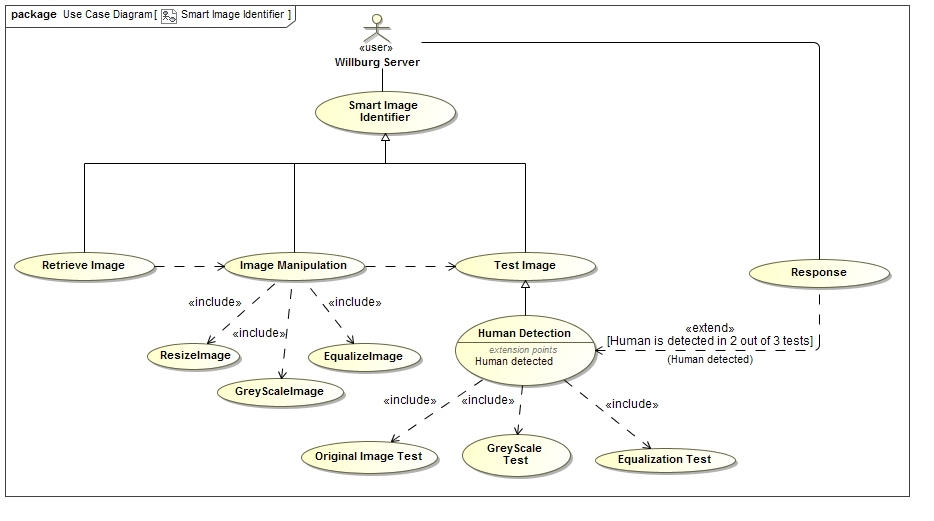
\includegraphics [scale=0.5]{../Diagrams/UML_Diagram.jpg}
		\caption{UML diagram of Smart Image Identifier}
	\end{figure}	
	\FloatBarrier

	\newpage
	\subsection {Service Contract}
	\begin{figure}[htb]
		\centering
		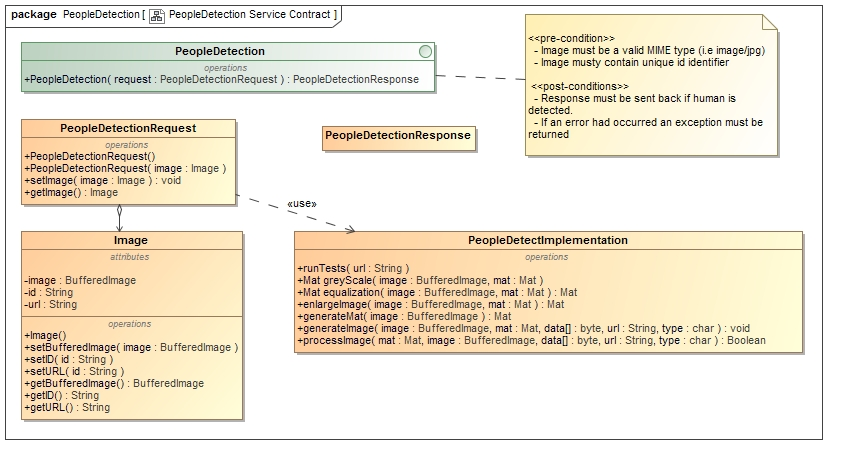
\includegraphics [scale=0.5]{../Diagrams/PeopleDetection_Service_Contract.jpg}
		\caption{Service contract of Smart Image Identifier}
	\end{figure}	
	\FloatBarrier

\newpage
	\subsection {Domain model}
	\begin{figure}[htb]
		\centering
		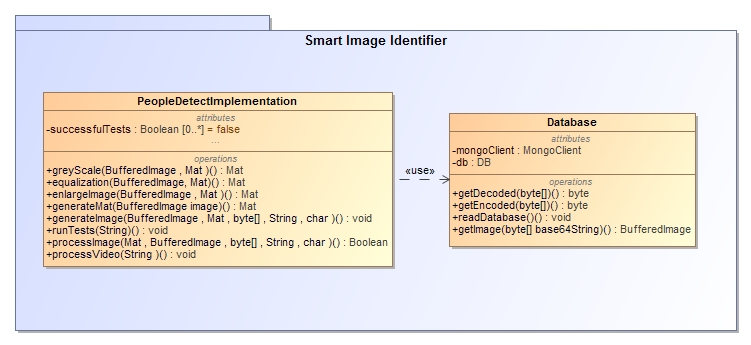
\includegraphics [scale=0.5]{../Diagrams/Model.jpg}
		\caption{Domain model of Smart Image Identifier}
	\end{figure}	
	\FloatBarrier
	


\section {Retrieve Image}
The Retrieve Image Service module is responsible for pulling images from the Willburg server for the system to process. The module will retrieve these image using an port connection to the server. Once these images are retrieved they are then assigned for testing.
	\FloatBarrier
	\subsection {Scope}
		The scope for the Retrieve Image Service module is shown in Figure4.
		\begin{figure}[htb]
			\centering
			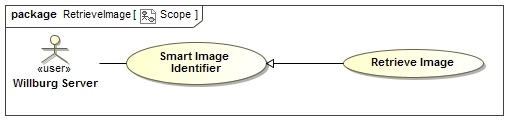
\includegraphics [scale=0.5]{../Diagrams/RetrieveImageScope.jpg}
			\caption{Retrieve Image scope}
		\end{figure}	
		\newpage
		The scope of the Retrieve Image module include:
			\begin {itemize}
				\item Retrieve image from the Willburg server.
				\item Assign image for testing.
			\end {itemize}

	\subsection {Retrieve Image service model conditions}
		\subsubsection {Pre-conditions}
			\begin {itemize}
				\item System must have a valid connection to the server. 
				\item Images must be of valid MIME type image
			\end {itemize}
		\subsubsection {Post-Conditions}
			\begin {itemize}
				\item Image is pulled from server and assigned for processing. 
			\end {itemize}
If there is an invalid connection to the to the server a NoConnection exception is thrown. If an error occurs during retrieval of the image an IOException is thrown.
			
		
		
		\subsection {Functional requirements}
The lower level services required by the retrieve image service to either check the pre-conditions or address the post-conditions is shown 2.

		\newpage
		\FloatBarrier
		\subsection {processDesign}
		The images are retrieved from the Willburg server in a base64 encoded string. The images are then decoded into a BufferedImage object. A Image object is created to store the id of the image and the BufferedImage object. The Image object is then sent as request to identify the presence of a human using the PeopleDetectionRequest object.
		\FloatBarrier
		\begin{figure}[htb]
			\centering
			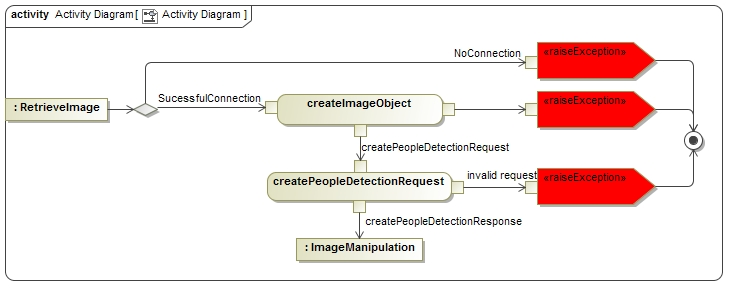
\includegraphics [scale=0.5]{../Diagrams/RetrieveImage_ActivityDiagram.jpg}
			\caption{Process image process design}
		\end{figure}	
		\FloatBarrier


	
	\section {Image Manipulation}
	\hfill \break
The Image Manipulation Service module is responsible for manipulating images inorder to better identify human. The module will manipulate each image by resizing the image, grayscaling and equalization. Once these images are manipulated they are then assigned for testing.
		\subsection {Scope}
			The scope for Image Manipulation Service module is shown is Figure 6.
			\begin{figure}[htb]
				\centering
				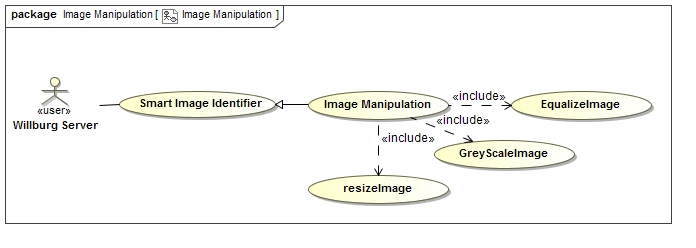
\includegraphics [scale=0.5]{../Diagrams/ImageManipulation_Scope.jpg}
				\caption{Image Manipulation scope}
			\end{figure}	
			\FloatBarrier

		\subsection {processDesign}
		The BufferedImage data is retrieved from the Image object, that was sent through in the request. The BufferedImage is then used to create three Mat obejcts. The first mat object is the original image itself. This mat object isthen resized and used to create the last two mat object. The second mat object is a grayscaled mat object and the third is the grayscaled mat object that was equalised. After these three mat objects are created they are sent on to the Test Image Service model for testing.
			\FloatBarrier
			\begin{figure}[htb]
				\centering
				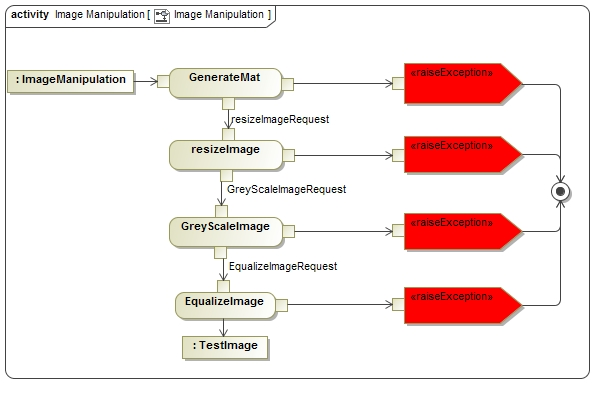
\includegraphics [scale=0.5]{../Diagrams/ImageManipulation_ActivityDiagram.jpg}
				\caption{Image Manipulation process design}
			\end{figure}	
			\FloatBarrier

	\newpage
	\section {Test Image}
		The Image Manipulation Service module is responsible for human detection. The module will use the manipulated image and the prerform human detection. The module will use the manipulated mat objects to perform three individual tests. These tests include performing human detection on the original image, grayscaled image and the equalised image.
		\subsection {Scope}
			The scope for Test Image Service module is shown is Figure 8.
			\begin{figure}[htb]
				\centering
				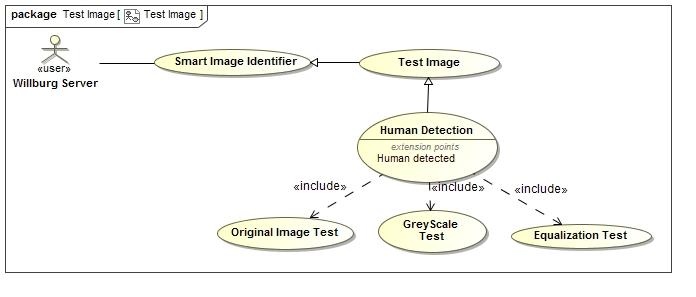
\includegraphics [scale=0.5]{../Diagrams/TestImage_Scope.jpg}
				\caption{Test Image scope}
			\end{figure}	
			\FloatBarrier
		
		\subsection {processDesign}
			The three manipulated mat objects are used to in a three phase test system inorder to improve the accuracy of human detection. Humand detection will be performed on each manipulated image. If two out of the three test are positive then the system has detected a human and a reponse will be sent to the server.
			\FloatBarrier
			\begin{figure}[htb]
				\centering
				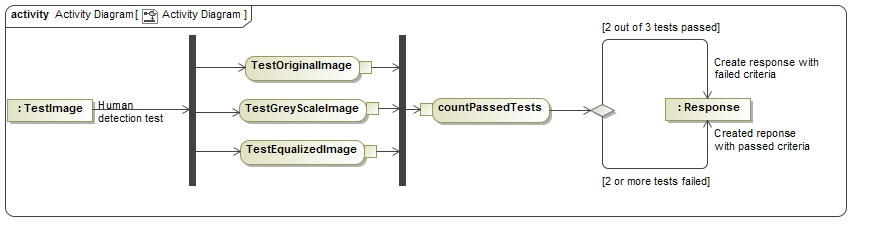
\includegraphics [scale=0.5]{../Diagrams/TestImage_ActivityDiagram.jpg}
				\caption{Test Image process design}
			\end{figure}	
			\FloatBarrier

	\section {Response}
		The Response Service module is creating a response object to send to the Willburg server.
		\subsection {Scope}
		The scope for Response Service module is shown is Figure 10.
			\begin{figure}[htb]
				\centering
				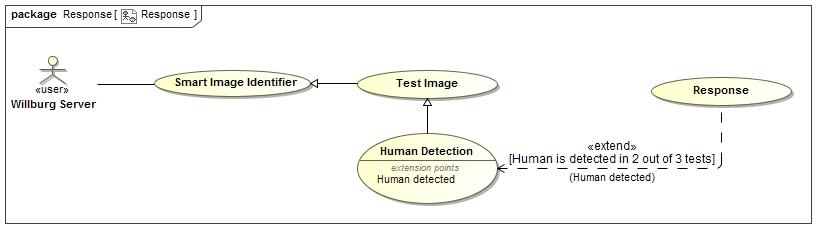
\includegraphics [scale=0.5]{../Diagrams/Response_Scope.jpg}
				\caption{Response scope}
			\end{figure}	
			\FloatBarrier
		
		
		\subsection {processDesign}
			A response object is created and sent back to the server.
			\FloatBarrier
			\begin{figure}[htb]
				\centering
				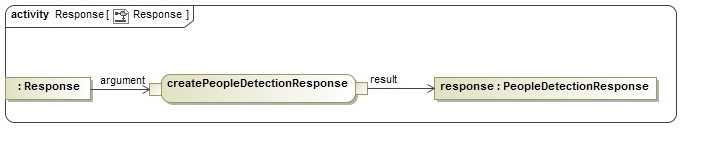
\includegraphics [scale=0.5]{../Diagrams/Response_ActivityDiagram.jpg}
				\caption{Response process design}
			\end{figure}	
			\FloatBarrier
\end{document}
